\documentclass[a4paper,11pt]{article}

%%%%%%%%%%%%%%%%%%%%%%%%%%%%%%%%%%%%%%%%%%
%            Packages                    %
%%%%%%%%%%%%%%%%%%%%%%%%%%%%%%%%%%%%%%%%%%
\usepackage{amsfonts}
\usepackage{amsmath}
\usepackage{amssymb}
\usepackage{graphicx}
\usepackage{comment}
% grafic preferences
\usepackage{graphicx,epic,eepic}
\usepackage{subcaption}
\usepackage{placeins}
\usepackage{floatrow}
\usepackage{pdfpages}
\usepackage{eso-pic}
\usepackage{lscape}
% pagestyle preferences
\usepackage{a4wide}
\usepackage{fancyhdr}
% SI units
\usepackage[squaren]{SIunits}
% Math formuals and stuff
\usepackage{amsmath}
\usepackage{amssymb}
\usepackage{amsfonts}
\usepackage{mathrsfs}
% Index
\usepackage{makeidx}
%\usepackage[
%top    = 2.8cm,
%bottom = 3.0cm]{geometry}
% LaTeX symbol
\usepackage{latexsym}
\usepackage{hyperref}
\urlstyle{same}
\usepackage{makeidx}
\usepackage{pdfpages}
\usepackage{textcomp}
\usepackage{eurosym}
\usepackage[a4paper,top=2cm]{geometry}

%%%%%%%%%%%%%%%%%%%%%%%%%%%%%%%%%%%%%%%%%%
%            Page style                  %
%%%%%%%%%%%%%%%%%%%%%%%%%%%%%%%%%%%%%%%%%%

%%%%%%%%%%%%%%%%%%%%%%%%%%%%%%%%%%%%%%%%%%
%            main body                   %
%%%%%%%%%%%%%%%%%%%%%%%%%%%%%%%%%%%%%%%%%%
\begin{document}
\pagenumbering{roman}
\title{Project: Gender Classification from Blog Data with Machine Learning}
\author{Rasmus Eriksen, Rikke Randl\o v \& Sofie Janas}
\maketitle
\tableofcontents
\newpage
\pagenumbering{arabic}
\section{Introduction}
Classifying large amounts of data is increasingly important in the modern, digital society, and methods such as data mining allows one to extract data from diverse regions. An important tool in classifying data are various methods within machine learning, such as boosted decision trees and support vector machines. We will utilize these two tools for gender classification and prediction for a large dataset of internet blogs collected by the authors of \cite{data}.

\section{Previous studies}
Classification of various personal information (gender, age, personality type, political leanings) is a large and ongoing research topic within fields such as machine learning and linguistics. Previous studies we have read (\cite{data}, \cite{other}) have utilized a large number of different predictors to determine the gender of the blog's author. The predictors includes various stylistic features (number of posts, number of characters in posts, posting frequencies etc.) and content-related features (special recurring words, occurences of verbs, adjectives, personal pronouns etc). Armed with these predictors, studies show accuracies of  62-89\% with various methods \cite{other}.

\section{Data set}
\label{sec:data}
The data set used in this project is 18.548 blogs, which contains, along the actual content of the blogs, also associated values of the bloggers' gender, age, occupation and zodiac. The blogs have been collected from the site blogger.com in august 2004. Each blog contains all posts the blogger has written up until the sampling date. We wish to use the classification tool to be able to consistently identify the gender of the blogger. It should be noted, that we only have data from bloggers in the age intervals: 13-17, 23-27 and 33-42.\\

\noindent When analysing the blogs with the intention of identifying the gender of the author, we need a set of predictors to run the learning algorithms on. Here we have two kinds of data: we have meta data, giving us the gender, age and job; and we have the actual blog, from which we can run a set of summary statistics on.
The meta data itself is applicable to the learning algorithm with minor modifications: The genders "male" and "female" can be directly translated into the binary labels $(1,2)$. The age does not need any translation and can be used directly. The jobs are pre-processed into 40 categories, and here each category can be assigned a label $(1,2,\dots,40)$.

\noindent This gives us the first 2 predictors:
\begin{enumerate}
	\item[1)] Age\vspace{-1em}
	\item[2)] Job
\end{enumerate}

\noindent For summary statistics we choose a few simple statistics, and a few more elaborate, and we will later consider the effectiveness of these statistics. The summary statistics give 11 additional predictors.
\begin{enumerate}
	\item[3)] The average post length (measured in number of characters)\vspace{-1em}
	\item[4)] The average word length (measured in number of characters)\vspace{-1em}
	\item[5)] The average posting frequency\vspace{-1em}
	\item[6)] The percentage of "Descriptors" (defined below)\vspace{-1em}
	\item[7)] The average number of URL links per post\vspace{-1em}
	\item[8)] The percentage of "Internet Words" (defined below)\vspace{-1em}
	\item[9-13)] The percentages of the words: \{"the", "i", "him", "of", "and"\}
\end{enumerate}

\noindent In the above section "Internet Words" are defined to be from the following list:
(lol, wtf, wth, dafuq, rofl, omg, brb, btw, irl, imo, jk, np, thx, imho, bae, bff, gr8, fml, l8r, yolo, swag, fyi, nvm, glhf, lulz, tbh, fail, 404, xoxo, stfu, 1337, noob, afaik, iou, asap, asl, w00t, cu, cya, ffs, fml, tmi, ftw, fu, derp, gtfo, haxor, idk, srsly, tldr, m8, sext, troll, sk8, sk8r, ty)

\noindent And "Descriptors" are defined as words ending with\cite{other}:
(able, al, ful, ible, ic, ive, less, ly, ous).\\

\noindent The distribution and correlations of the predictor data is shown in figure \ref{fig:DataDistributions} as a corner plot: in the diagonal histograms of the 8 predictors are plotted, and in the sub-diagonal is shown the 2D correlation plots between parameter $i$ and $j$. It is obvious that none of the 8 predictors seem to separate the data very well on their own.\\

\noindent We will also train the adaptively boosted decision tree using the predictors 1-13, with the last 5 predictors having a cornerplot as shown in figure \ref{fig:Corner_word}
\FloatBarrier
\begin{figure}[h!]
   %\centering
    \centerline{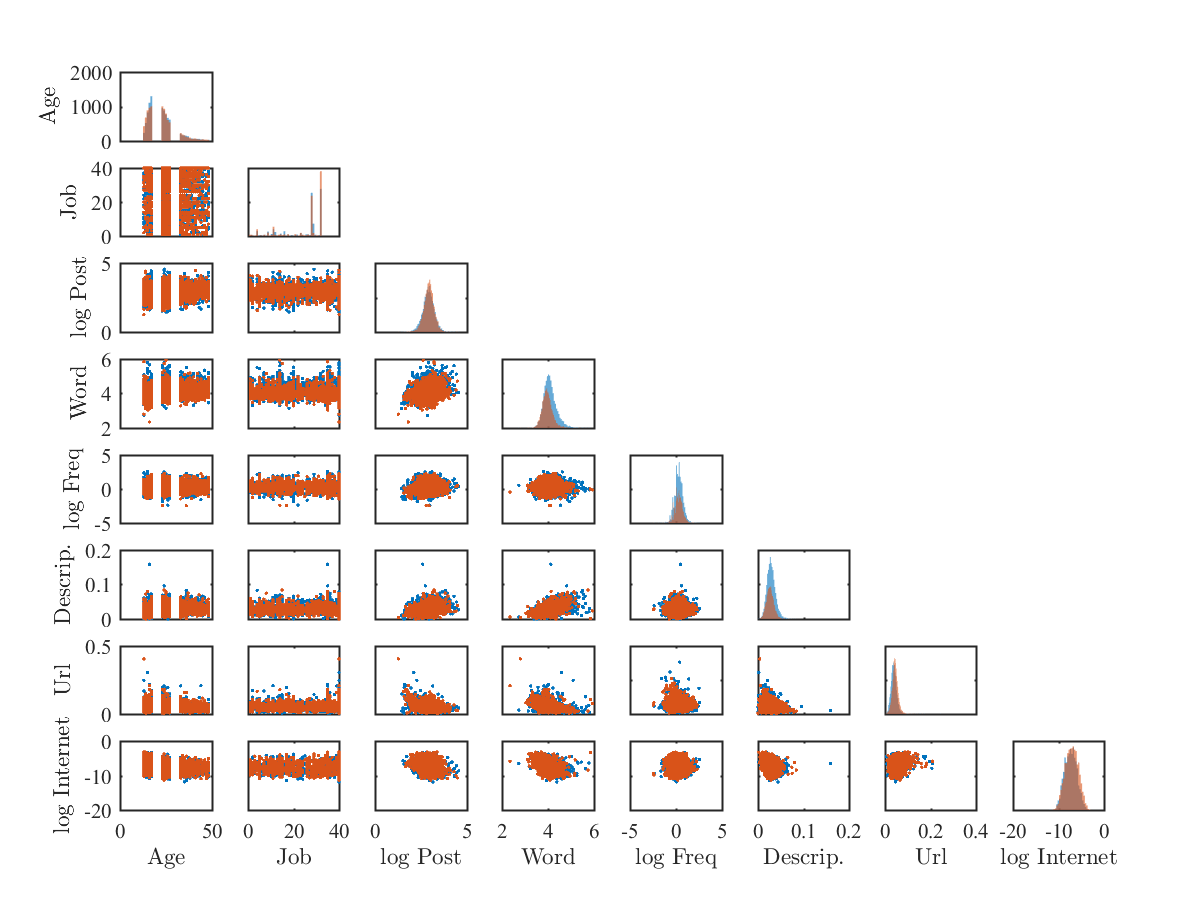
\includegraphics[width=1.2\textwidth]{Pix/Corner.png}}
    \caption{Corner plot of the predictors 1-8 from above. Red indicates female, and blue indicates male. The diagonal shows the histogram of each predictor, whereas the plot ($i$,$j$) is the correlation between predictor $i$ and $j$. For the predictors average post length, frequency and percentage of "internet words" the logarithm of that predictor is shown instead for ease of view. (A larger plot of the figure can be seen after the references).}
    \label{fig:DataDistributions}
   	\vspace{-1em}
\end{figure}

\begin{figure}[h!]
   %\centering
    \centerline{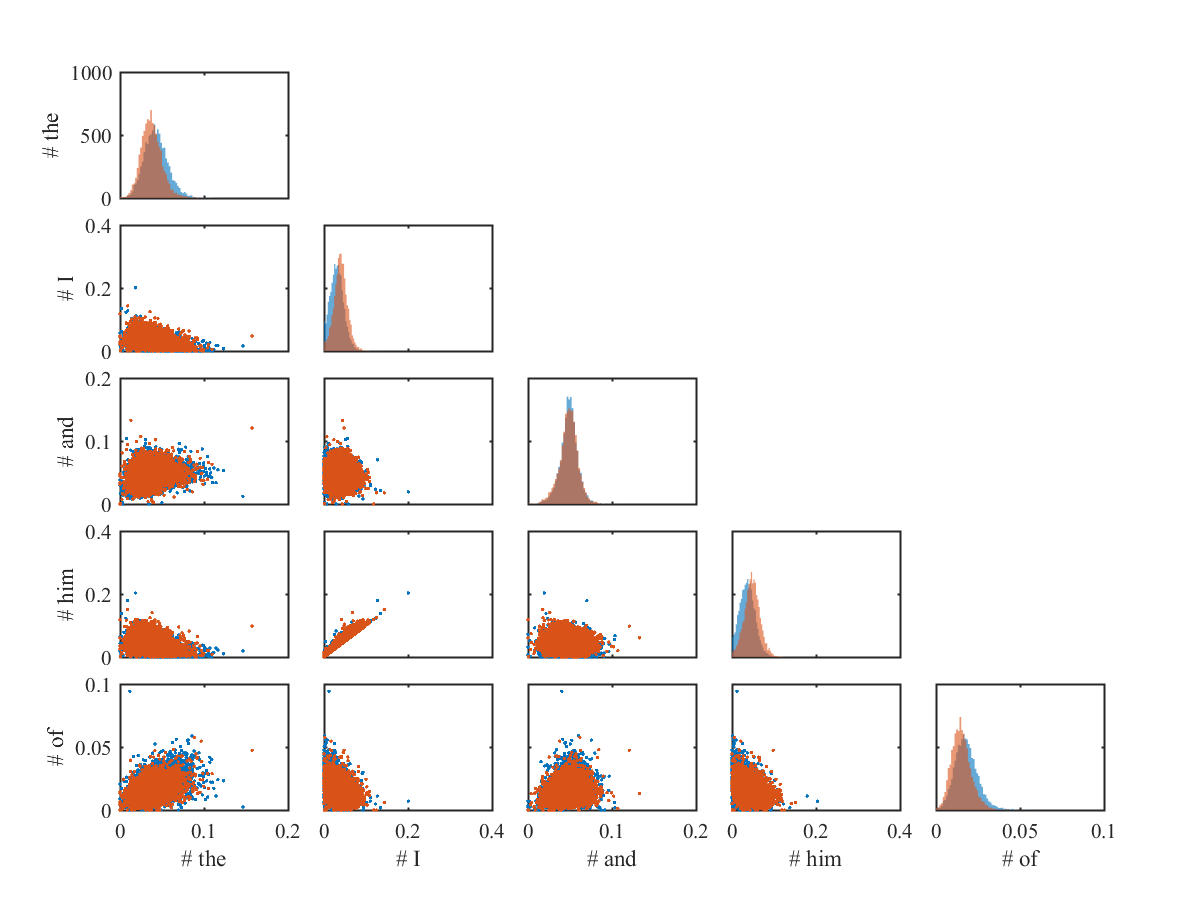
\includegraphics[width=1\textwidth]{Pix/Corner_word.png}}
    \caption{Corner plot of the predictors 9-13 from above. Red indicates female, and blue indicates male. The diagonal shows the histogram of each predictor, whereas the plot ($i$,$j$) is the correlation between predictor $i$ and $j$.}
    \label{fig:Corner_word}
\end{figure}
\FloatBarrier
\section{Methods}
\noindent There are various methods within machine learning, but in this project we will compare two methods, namely decision trees with adaptive boosting (AdaBoost) and support vector machines (SVM).

\subsection{Decision trees with adaptive boosting}
Boosted decision trees is a variant of the decision tree algorithm, which uses an iterative method to account for misclassification of the previous iteration.
The first "generation" of the boosted decision tree is just a regular decision tree; the "boosting" in the algorithm comes by re-weighing the data-points after the decision tree algorithm has been applied. The data-points are re-weighted such that the misclassified points are given extra weight (the weights of correctly-classified points do not change), and this extra weight makes it more likely that the decision tree algorithm, when run again, will correctly label these re-weighted points (at the cost of now miss-classifying other points). Each iteration of this algorithm is stored as a generation of the tree, and by repeating the steps the boosted decision tree is grown. The final classification is then made by taking the combined output of all generations; this output is a fuzzy-logical value for the probability that a given data-point has a given label, and the final classification step is then decided by the threshold value chosen by the user.
\noindent In this case, as we are equally interested in the two classes, the threshold value is set to 50 \%.

\noindent The adaptive boosting method describes a way of re-weighing misclassified points, and a way of combining the outputs of each generation, but we will not describe this in detail, as the choice for the specific boosting method is somewhat arbitrary, and any other method, such as LogitBoost, could have been used.
\subsection{Support vector machines}
For this project we will also use a Support Vector Machine (SVM); specifically we will use a Soft-Margin SVM. which is a type of SVM which allow for some slack in the separation of data-points. The SVM works by detecting the best possible (hyper)plane that separates the data-points; in the simple case, where the data is linearly separable, this is just a regular (hyper)plane in feature space. However, if the data is not linearly separable one can instead use the so-called kernel methods to transform the data from the feature space to a higher dimensional space, use a (hyper)plane to separate the now linearly-separable data, and transform the data back into feature space, where the resulting decision boundary is not necessarily linear in this space. This allow for some highly complex decision boundaries which can (hopefully) separate the data convincingly.\\

\noindent This method does come at a cost however, since we need to tune some of the parameters of the SVM to give the optimal results: The slack-parameter $C$ and a kernel parameter $\sigma$. The slack parameter is a regularizer for how much we allow points to be misclassified, and the kernel parameter is (in this case) the width of the Gaussian kernel used to transform the data. There are other choices for the basis function of the transformation, but the Gaussian is easy and robust.
\noindent The tuning of the parameters is done by five-fold cross-validation of the training data%; this entails splitting the training data into 5 sets, and systematically forming 5 new sets with one of the subsets left out. Then 
, and the set of values for $C$ and $\sigma$ which has the lowest cross-validation loss is chosen as the SVM parameters.
\section{Results}
\FloatBarrier
\noindent Using the boosted decision trees with the AdaBoost method, we grow our decision tree using the first 8 predictors - that is we did not train the tree on the frequencies of the five test words. We use 50\% of the data to grow the tree, and the remaining data for testing. The resulting separation of the test data by the decision tree is shown in figure \ref{fig:AdaBoost8}. The accuracy of the decision tree is 63.4\%.
%\begin{figure}[h]
%\centering
%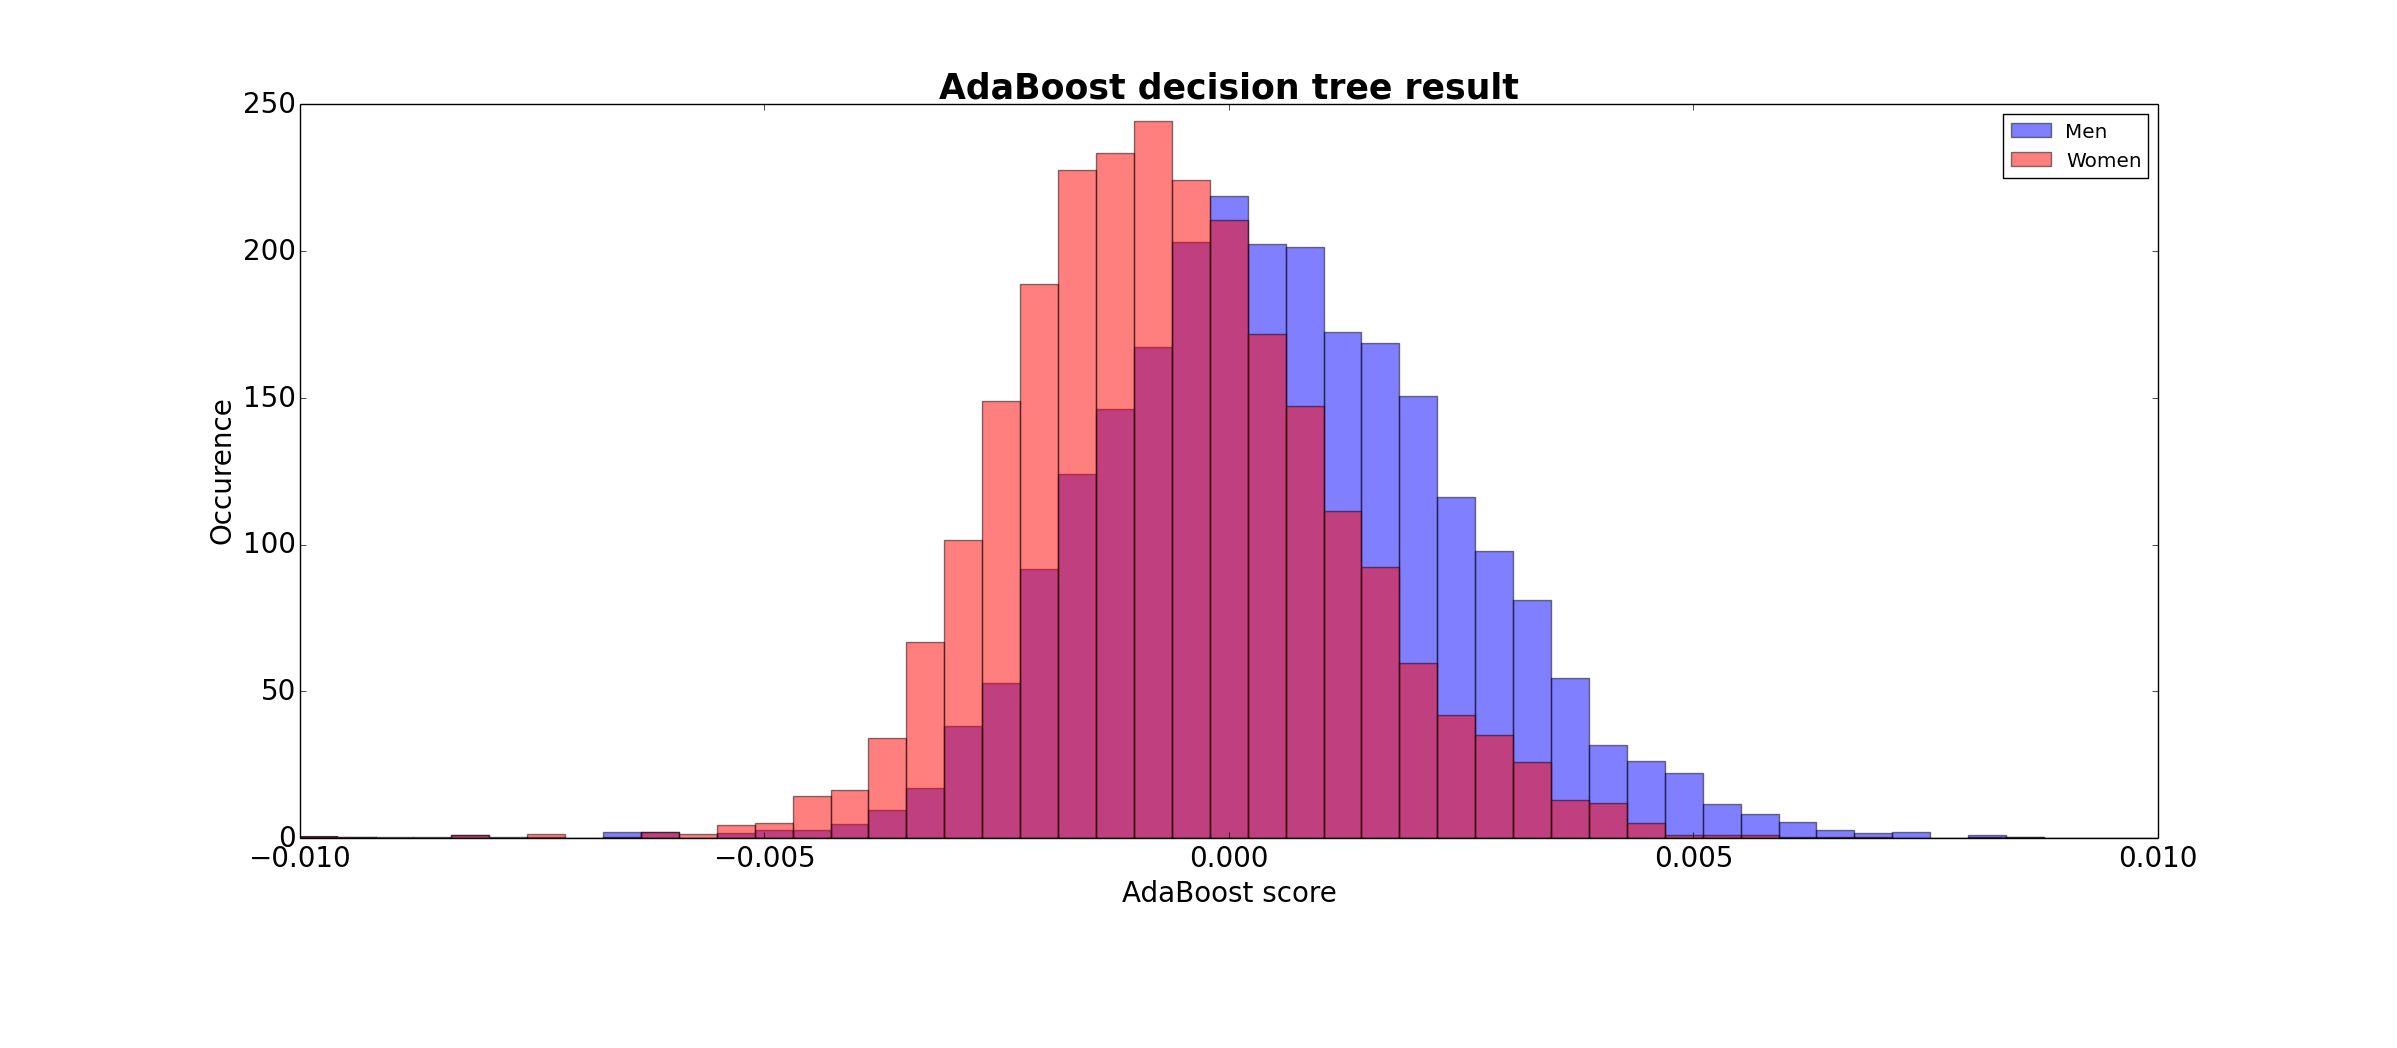
\includegraphics[width=\textwidth]{Pix/HistAdaB8.png}
%\caption{The separation of the test data using the AdaBoost method and predictors 1-8. The tree is grown using 50\% of the data set and remaining 50\% is the test data. A value smaller (larger) than zero corresponds to the label "female" ("male")}
%\label{fig:AdaBoost}
%\end{figure}

\noindent We also run the algorithm using all 13 predictors, and again we use 50\% of the data to grow the tree. The results using these predictors is shown in figure \ref{fig:AdaBoostAll}. The accuracy of the decision tree is here 65.8\%.
%\begin{figure}[h]
%\centering
%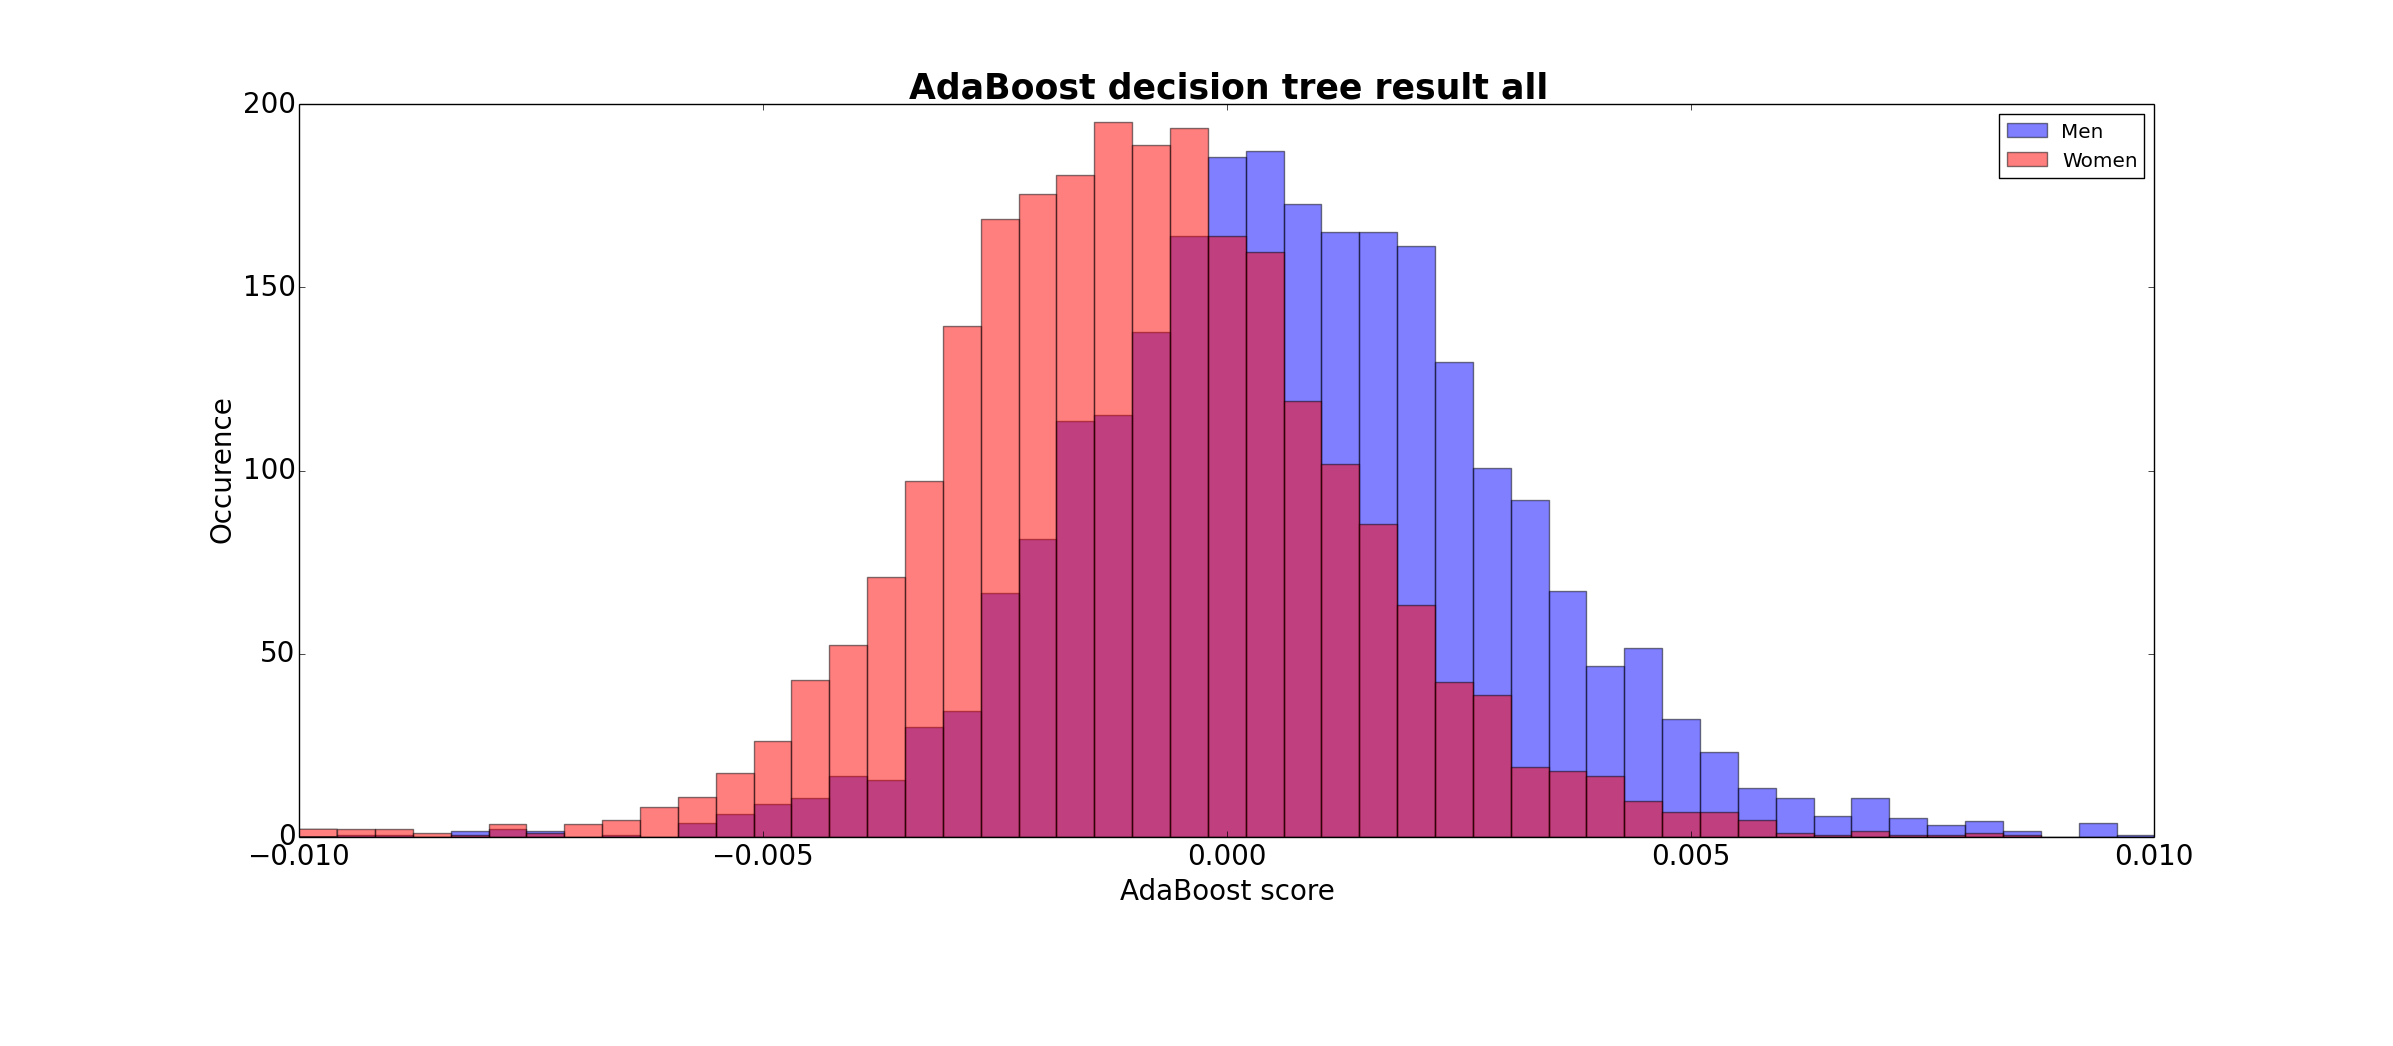
\includegraphics[width=\textwidth]{Pix/HIstAdaAll.png}
%\caption{The separation of the test data using the AdaBoost method and predictors 1-13. The tree is grown using 50\% of the data set and remaining 50\% is the test data. A value smaller (larger) than zero corresponds to the label "female" ("male")}
%\label{fig:AdaBoostAll}
%\end{figure}

\begin{figure}[h]
    \centering
    \begin{subfigure}[b]{0.45\textwidth}
        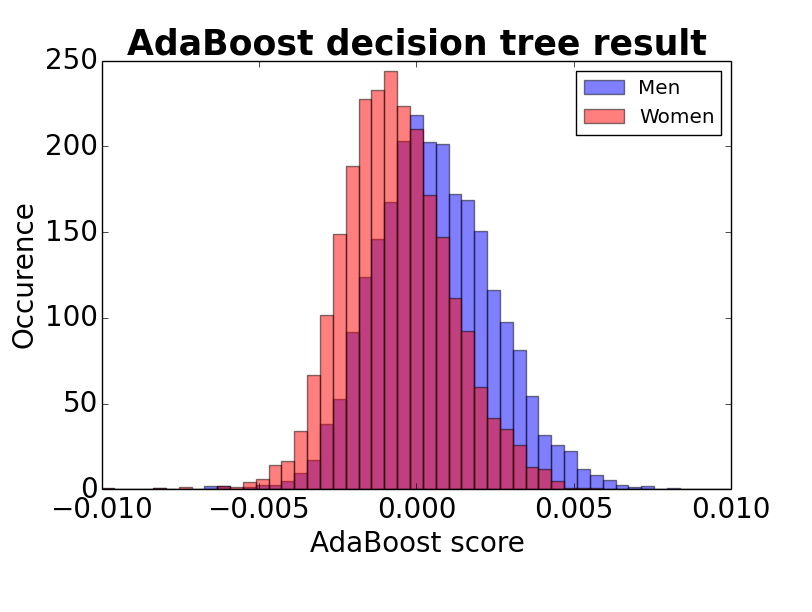
\includegraphics[width=\textwidth]{Pix/HistAdaB82.png}
		\caption{The separation of the test data using the AdaBoost method and predictors 1-8. This yields an accuracy of 63.4\%.}
		\label{fig:AdaBoost8}
    \end{subfigure}
    ~
    \begin{subfigure}[b]{0.45\textwidth}
		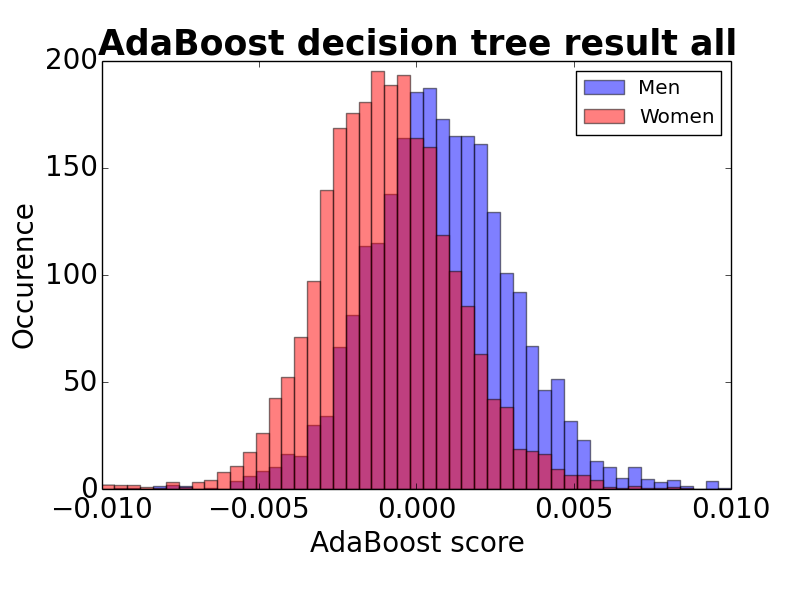
\includegraphics[width=\textwidth]{Pix/HIstAdaAll2.png}
		\caption{The separation of the test data using the AdaBoost method and predictors 1-13. This yields an accuracy of 65.8\%.}
		\label{fig:AdaBoostAll}
    \end{subfigure}
    \caption{The tree is grown using 50\% of the data set and remaining 50\% is the test data. A value smaller (larger) than zero corresponds to the label "female" ("male"). The colors of the two histogram corresponds to the true label.}
	\label{fig:AdaBoost}
\end{figure}
\noindent We now look at the importance of each of the predictors in both cases. This is shown in figure \ref{fig:imprtances}.  Note that the frequency of three of the five test words rank highly when using all 13 predictors, suggesting that some contextual linguistic features in the data set are more important many of more descriptive ones (such as average word length  etc.).\\

\begin{figure}[h!]
   %\centering
    \centerline{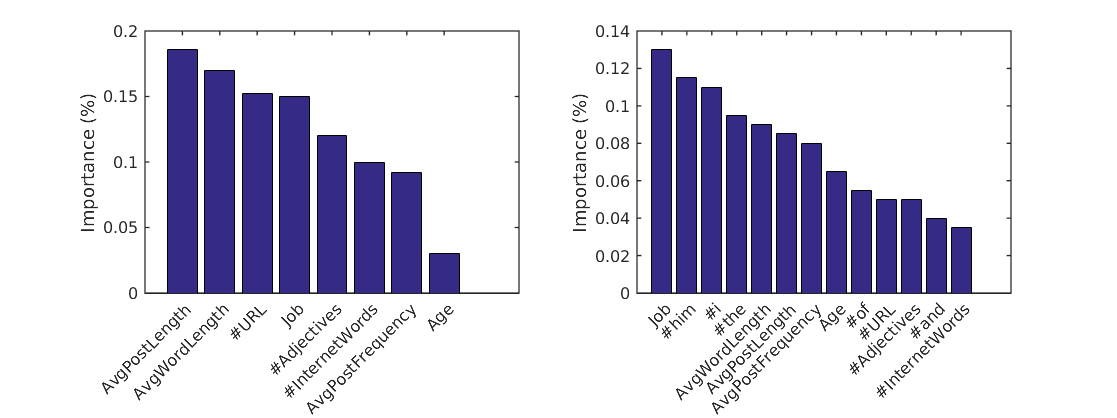
\includegraphics[width=1\textwidth]{Pix/ParameterImportance.png}}
    \caption{The importance of each of the predictors. On the left, we use the first 8 predictors, and on the right we use all 13 predictors.}
    \label{fig:imprtances}
\end{figure}
\noindent For this project we also trained an SVM for comparison with the AdaBoost method. Here we used the predictors 1-8.
With these 8 predictors, we train the SVM on 20\% of the data, and use the remaining 80\% of the data as test data. The 5-fold cross-validation error on the training sample is shown in figure \ref{fig:SVM_02}; the smallest cross-validation error is found for $(C,\sigma) = (10^2,10)$. The scores of the test data generated by the SVM is shown in figure \ref{fig:SVM_02_score}, with an accuracy on the test data of 62.4\%.\\

\noindent To illustrate the role of the division of training and test data, we train the SVM again now using 50\% of the data as training data. The associated 5-fold cross validation error plot is shown in figure \ref{fig:SVM_05}; now with the lowest cross-validation error for $(C,\sigma) = (10,10^4)$. The SVM score is shown in figure \ref{fig:SVM_05_score}; the increase in training data does only improves the performance by about one percent, as the accuracy on the test data is now 63.5\%.

\begin{figure}[h]
    \centering
    \begin{subfigure}[b]{0.45\textwidth}
        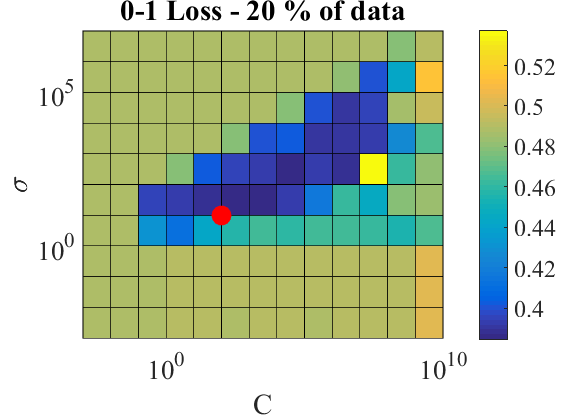
\includegraphics[width=\textwidth]{Pix/SVM_02_fixd.png}
		\caption{Using 20\% of the data as training data. Minimum loss found is 0.362 at (C,$\sigma$)=(100, 10).}
		\label{fig:SVM_02}
    \end{subfigure}
    ~
    \begin{subfigure}[b]{0.45\textwidth}
        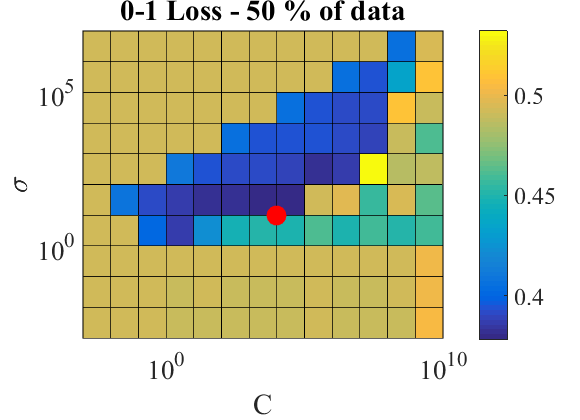
\includegraphics[width=\textwidth]{Pix/SVM_05_fixd.png}
		\caption{Using 50\% of the data as training data. Minimum loss found is 0.350 at (C,$\sigma$)=(10, $10^4$).}
		\label{fig:SVM_05}
    \end{subfigure}
    \caption{The five-fold cross-validation loss of the SVM as a function of the parameters $C$ and $\sigma$. The red point shows the minimum loss, and the corresponding values of the parameters are used for the final SVM}
	\label{fig:SVM_Train}
\end{figure}

\begin{figure}[h]
    \centering
    \begin{subfigure}[b]{0.45\textwidth}
        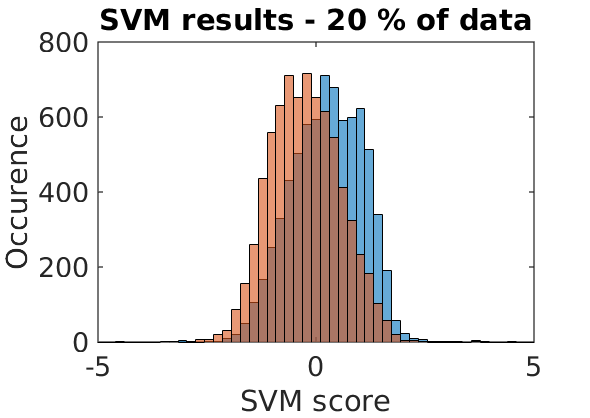
\includegraphics[width=\textwidth]{Pix/SVM_02_Score.png}
		\caption{Using 20\% of the data as training data. This yields an accuracy of 62.4\%.}
		\label{fig:SVM_02_score}
    \end{subfigure}
    ~
    \begin{subfigure}[b]{0.45\textwidth}
        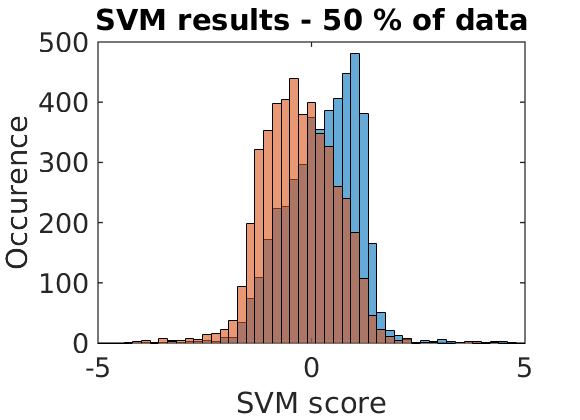
\includegraphics[width=\textwidth]{Pix/SVM_05_Score.png}
		\caption{Using 50\% of the data as training data. This yields an accuracy of 63.5\%.}
		\label{fig:SVM_05_score}
    \end{subfigure}
    \caption{The separation of the two genders in terms of their SVM score using predictors 1-8. A value smaller (larger) than zero corresponds to the label "female" ("male").}
	\label{fig:SVM_Result}
\end{figure}
\FloatBarrier

\section{Discussion}
\noindent For both the SVM and the AdaBoost using predictors 1-8 the accuracy is found to be around 63.4\% - 63.5\%, though the shape of the histograms in figures \ref{fig:AdaBoost8} and \ref{fig:SVM_05_score} is not completely alike. That the two algorithms agree to closely is hardly surprising, but it is satisfying that both yield the same results. There is however a clear runtime difference between SVM and AdaBoost: SVM requires extensive tuning, which has a rather large runtime on the order of 16 hours in our laptops, with AdaBoost being significantly faster as it requires no tuning of parameters - thus AdaBoost is also parameter-free, another advantage.\\

\noindent The best prediction accuracy we obtain is $\sim$ 66\%, which is hardly impressive when compared to the best results from the articles we have read, which can come close to 89\% \cite{other}. However, the large difference seems to come from the fact that their predictors have been based largely on clever linguistic choices (writing styles parametrized in some clever way, etc.), which we do not have the linguistic knowledge to repeat.\\

\noindent Also interesting is the fact that the SVM's performance does not increase significantly with more training data after 20\%. This suggest that the generalization potential has been reached, meaning that the algorithm does not become significantly better at generalizing as it gets more data.
We saw a similar effect in the AdaBoost algorithm (an increase of about one percent), but we have not shown it in this project.\\

\noindent Using all 13 predictors for the AdaBoost algorithm increases the accuracy to 65.8\%, a slight improvement of 2.4\%. That such clear seperation in 5 very common words exists (as shown in figure \ref{fig:Corner_word}) is somewhat surprising, but may reflect on the formal vs contextual writing style which is apparently distinctive in the two genders \cite{data}. Investigating the parameter space for all 13 predictors with the SVM proved too big a runtime challenge for the deadline of this project.

\section{Conclusion}
We have used the machine learning algorithms boosted trees with adaptive boosting (adaBoost) and support vector machines (SVM) to attempt a gender classification on a dataset of more than 15,000 blogs. Using 8 predictors (defined in section \ref{sec:data}) the two algorithms yield nearly the same separation of data with an accuracy of 63.4\% for adaBoost and 63.5\% for SVM, indicating that the two algorithms perform equally well on our data, though SVM has a significantly larger runtime. An additional training has been run using all 13 predictors using adaBoost, which improved the accuracy up to 65.8\%. These rates are significantly better than blind guesses, though not nearly as well as the best in literature \cite{other}.


\begin{thebibliography}{9}

\bibitem{data}
	J. Schler, M. Koppel, S. Argamon \& J. Pennebaker,
	\textit{Effects of Age and Gender on Blogging},
	, Proc. of the Association for the Advancement of Artificial Intelligance (March 2006)

\bibitem{other}
A. Mukherjee \& B. Liu,
\textit{Improving Gender Classification of Blog Authors},
Proceedings of the 2010 Conference on Empirical Methods in Natural Language Processing, p. 207–217, 2010

\end{thebibliography}

\newpage
\newgeometry{left=1cm,right=1cm,top=1cm,bottom=1cm}
\begin{landscape}
\begin{figure}[h]
   %\centering
    \centerline{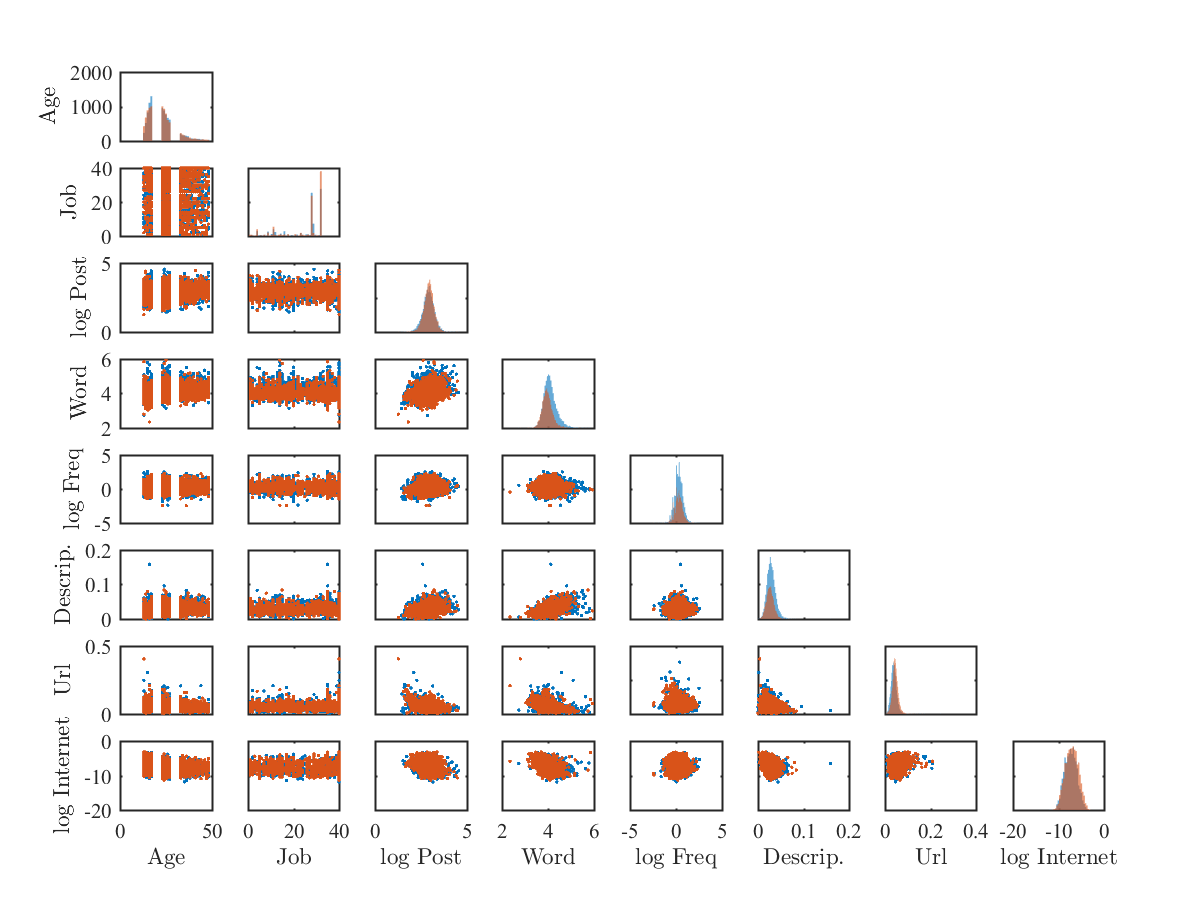
\includegraphics[width=0.9\textwidth]{Pix/Corner.png}}
    \caption{Corner plot of the predictors 1-8 from above. Red indicates female, and blue indicates male. The diagonal shows the histogram of each predictor, whereas the plot ($i$,$j$) is the correlation between predictor $i$ and $j$.}
    \label{fig:Huge}
\end{figure}
\end{landscape}

\end{document}

%\begin{figure}
%\centering
%\subfigure[Age]{\includegraphics[width=0.3\textwidth]{Pix/Age.jpg}
%\label{fig:subfigure1}}
%~
%\subfigure[Entires]{\includegraphics[width=0.3\textwidth]{Pix/Entries.jpg}
%\label{fig:subfigure2}}
%~
%\subfigure[Frequency]{\includegraphics[width=0.3\textwidth]{Pix/Frequency.jpg}
%\label{fig:subfigure3}}
%~
%\subfigure[Word length]{\includegraphics[width=0.3\textwidth]{Pix/Wordlength.jpg}
%\label{fig:subfigure4}}
%~
%\subfigure[Post length]{\includegraphics[width=0.3\textwidth]{Pix/Postlength.jpg}
%\label{fig:subfigure5}}
%~
%\subfigure[Zodiac]{\includegraphics[width=0.3\textwidth]{Pix/Zodiac.jpg}
%\label{fig:subfigure6}}
%~
%\subfigure[Job]{\includegraphics[width=0.6\textwidth]{Pix/Job.jpg}
%\label{fig:subfigure7}}
%%
%\caption{Histograms of the 7 variables. Blue indicates male, red indicates female bloggers.}
%\label{fig:DataDistributions}
%
%\end{figure}
